%\documentclass{report}\begin{document}
\chapter{Origin of the Rubik's Cube}

\myTop{In this chapter we will describe the history behind \erno{} and how he got the idea for the \rubik{} will be described in order to get at better understanding of it. 
%Furthermore we will look at the development and the problematics describing the patenting and legal issues regarding the cube. 
Furthermore the legal issues and the problematics in regards to the patenting of the \rubik{} will be described.
The purpose of this chapter is to give the reader a contextual perspective on the \rubik{}.}
\section{Ern\"{o} Rubik}
\erno{} is the inventor of the world famous \rubik{}. He was born in Budapest, Hungary in 1944. His father was a flight engineer and his mother was a poet. He graduated from the Technical University in Budapest as an architectural engineer. After his graduation he stayed at the university to teach interior design.

In \myDate{}{1}{1975} Rubik applied for a patent for his invention in Hungary that was originally made to help his students. Two years later in 1977 he got the patent on the \mcube{}. 
This \mcube{} is actually the same cube as todays \rubik{}, he just named it differently. 
His \mcube{} should not be confused with the \mcube{} described in section \ref{sub:mcube}.
\emph{ Der er et spring fra Magic Cube til Rubiks Cube, som ikke beskrives}

In the 1980's he became a professor and started the Rubik Studio, which employs a dozen people to design furniture and toys. 
Since the studios' opening Rubik has produced several other toys, including Rubik's Snake. Most recently  the studio began developing computer games. 
He also became the president of the Hungarian Engineering Academy in 1990. The same year he created the International Rubik Foundation to support especially talented young engineers and industrial designers.

\begin{figure}
	\centering
		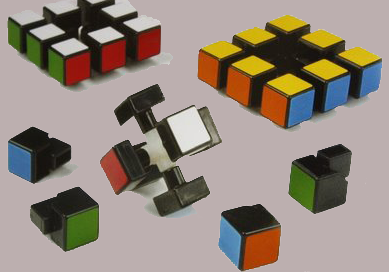
\includegraphics[scale=0.6]{input/pics/rubiks-cube.png}
	\caption{\myCaption{Figure of a disassembled Rubik's Cube.}}
	\label{fig:rubiks-cube}
\end{figure}
 
\section{Rubik's Cube}

%In the 70s \erno{} was teaching Interior Design at Academy of Applied Arts and Crafts and he was trying to find a tool to help his students to understand three dimensional objects. As result he made the \mcube{} in 1974 and obtained a Hungarian patent HU170062. 
% Det ovenover er allerede beskrevet i forrige section

In the 1970's when \erno{} was teaching at the university he wanted to create a tool that would help his students to better understand tree-dimensional design. 
He wanted a design with blocks that could be moved individually, but also able to move several blocks at a time. 
Initially he attempted to do this with a cube held together by rubber bands. 
This failed. 
He then concluded after looking at a  Magic Puzzle (see subsection \ref{sub:magicPuzzle}) that the pieces must hold each other in place. 
Thereby he created what was then called the \mcube{}. 

%Rubik described that some of the most important features behind the cube were that the parts of the cube stay together, which many other puzzles do not. He also pointed out that you can move several pieces at once. Also that it is three dimensional. 

In the end of 1970's a Hungarian Businessman showed the Magic Cube at the Nuremberg toy fair and made it popular in Europe. 
The company Ideal Toy bought exclusive rights for the Magic Cube, but changed the name of the cube to \rubik{} within a year in order to get trademark protection.

At that time there were also two others applying for patent for products similar to the \rubik{}.  
One of them was an American man named Doctor Larry D. Nichols and his cube was a 2x2x2 cube, which was held together with magnets. See section \ref{sec:nichols}. 
The other one who applied for patent was a Japanese man named Terutoshi Ishige. 
He applied for patent a year after \erno{}. 
Terutoshi Ishige's cube was almost identical to the \rubik{}.

Ideal Toy Company was bought by CBS Toy Company in 1982 and the trademark passed with it, but they sold the rights to \rubik{} to Seven Towns which is a toy company in Great Britain, and they are still producing the \rubik{} today.

\section{The Nichols Cube Puzzle}
\label{sec:nichols}
Dr. Larry D. Nichols studied chemistry at DePauw University in Greencastle, Indiana, before moving to Massachusetts to attend Harvard Graduate School. 
He is a lifelong puzzle enthusiast and inventor who  began developing a twist cube puzzle with six colored faces in 1957. 
It was made of eight smaller cubes assembled to a 2x2x2 cube. 
The eight cubes were held together by magnets.

\begin{figure}[htb]
	\centering
		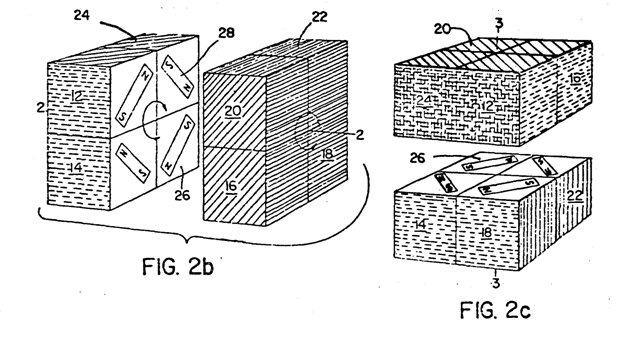
\includegraphics[scale=0.6]{input/pics/Nicholspatent2.png}
	\caption{\myCaption{Figure of Nichols Patent.}}
	\label{fig:Nicholspatent2}
\end{figure}

On \myDate{11}{4}{1972} he was granted U.S. Patent 3,655,201 on behalf of Moleculon Research Corp. U.S. Patent 3,655,201 covered Nichols Cube and the possibility for making larger versions later. 
This was two years before \erno{} took out the patent for his \rubik{} in Hungary. 

In 1982 Moleculon Research corp. sued Ideal Toy Company that had the U.S. Patent 4,378,116 for \rubik{} because they believed that Ideal Toy Company violated their patent, but the U.S. District Court ruled in Ideal Toy Company's favor. In 1986 the Court of Appeals ruled that the Pocket \rubik{} 2x2x2 was guilty of infringement but not the 3x3x3 \rubik{}. 

\begin{comment}
\myTail{In this chapter it has been described how \erno{} got the idea for the cube. We also stated that \erno{} was not the only one at that time, that came with the invention of cubes. \erno{}'s cube was special since the blocks hold each other together, which is different from the one Doctor Larry D. Nichols applied patent for which is hold together with magnets. 
}
\end{comment}
\myTail{
This chapter describes how \erno{} got the idea for the \rubik{}. 
It is also stated that \erno{} was not the only one with an idea of a cube shaped puzzle.
This chapter gives a better understanding and a contextual perspective of the creation of the \rubik{}.
}

%\end{document}